\documentclass{article}
\usepackage[a4paper, margin=1in]{geometry}  % Set uniform 1-inch margins
\usepackage{tikz}
\usetikzlibrary{arrows.meta}
\usetikzlibrary{calc} 
\usepackage{xcolor}
\usepackage{graphicx}
\definecolor{skyblue}{RGB}{135,206,250}
\usepackage{listings}
\title{Graph Practices}
\author{Sumaiya Tabassum}
\begin{document}


	\maketitle
\lstset{
 language=[LaTeX]TeX,           % Set LaTeX language
 basicstyle=\ttfamily\footnotesize,
    keywordstyle=\color{blue},
    stringstyle=\color{red},
    commentstyle=\color{green!60!black},
    numbers=left,
    numberstyle=\tiny\color{gray},
    stepnumber=1,
    numbersep=10pt,
    frame=single,
    showstringspaces=false,
    breaklines=true,
    tabsize=2      
}
	
\section{Practices:}

\subsection{Practice 01:}
\begin{lstlisting}
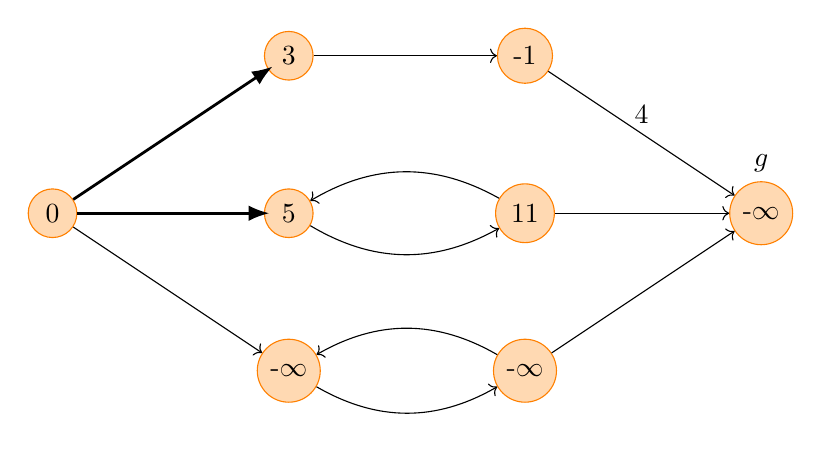
\begin{tikzpicture}
	\node(0) at (0,0)[circle,orange,fill= orange!30,text=black,draw]{0};
	\node(3) at (3,2)[circle,orange,fill= orange!30,text=black,draw]{3};
	\node(5) at (3,0)[circle,orange,fill= orange!30,text=black,draw]{5};
	\node(i1) at (3,-2)[circle,orange,fill= orange!30,text=black,draw]{-$\infty$};
	\node(-1) at (6,2)[circle,orange,fill= orange!30,text=black,draw]{-1};
	\node(11) at (6,0)[circle,orange,fill= orange!30,text=black,draw]{11};
	\node(i2) at (6,-2)[circle,orange,fill= orange!30,text=black,draw]{-$\infty$};
	\node(i3) at (9,0)[circle,orange,fill= orange!30,text=black,label=above:$g$,draw]{-$\infty$};
%\usetikzlibrary{arrows.meta}
	\draw[->, >=Latex, line width=1pt, shorten >=-2pt] (0) to (3);
	\draw[->, >=Latex, line width=1pt, shorten >=-2pt] (0) -- (5);
	\draw[->] (0) to (i1);
	\draw[->] (3) to (-1);
	\draw[->, bend right =30] (5) to (11);
	\draw[->,bend right =30] (11) to (5);
	\draw[->, bend right =30] (i1) to (i2);
	\draw[->,bend right =30] (i2) to (i1);
	\draw[->] (-1) to  node[midway, above]{4}(i3);
	\draw[->] (11) to (i3);
	\draw[->] (i2) to (i3);
				
\end{tikzpicture}
\end{lstlisting}
			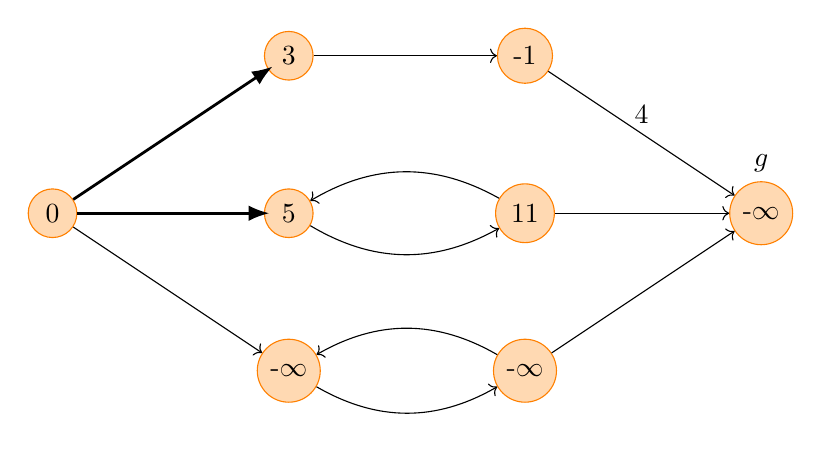
\begin{tikzpicture}
				\node(0) at (0,0)[circle,orange,fill= orange!30,text=black,draw]{0};
				\node(3) at (3,2)[circle,orange,fill= orange!30,text=black,draw]{3};
				\node(5) at (3,0)[circle,orange,fill= orange!30,text=black,draw]{5};
				\node(i1) at (3,-2)[circle,orange,fill= orange!30,text=black,draw]{-$\infty$};
				\node(-1) at (6,2)[circle,orange,fill= orange!30,text=black,draw]{-1};
				\node(11) at (6,0)[circle,orange,fill= orange!30,text=black,draw]{11};
				\node(i2) at (6,-2)[circle,orange,fill= orange!30,text=black,draw]{-$\infty$};
				\node(i3) at (9,0)[circle,orange,fill= orange!30,text=black,label=above:$g$,draw]{-$\infty$};
%\usetikzlibrary{arrows.meta}
				\draw[->, >=Latex, line width=1pt, shorten >=-2pt] (0) to (3);
				\draw[->, >=Latex, line width=1pt, shorten >=-2pt] (0) -- (5);
				\draw[->] (0) to (i1);
				\draw[->] (3) to (-1);
				\draw[->, bend right =30] (5) to (11);
				\draw[->,bend right =30] (11) to (5);
				\draw[->, bend right =30] (i1) to (i2);
				\draw[->,bend right =30] (i2) to (i1);
				\draw[->] (-1) to  node[midway, above]{4}(i3);
				\draw[->] (11) to (i3);
				\draw[->] (i2) to (i3);
				
			\end{tikzpicture}
\pagebreak		
		\subsection{Practice 02:}
\begin{lstlisting}
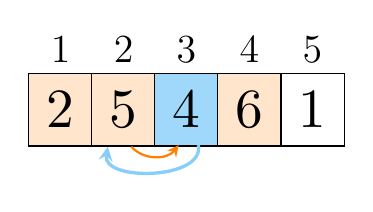
\begin{tikzpicture}
	\node(2) at (0,0)[text=black,fill=orange!20,label=\Large1,draw,scale=2]{2};
	\node(5) at (0.8,0)[text=black,fill=orange!20,label=\Large2,draw,scale=2]{5};
	\node(4) at (1.6,0)[text=black,fill=skyblue!80,label=\Large 3,draw,scale=2]{4};
	\node(6) at (2.4,0)[text=black,fill=orange!20,label=\Large 4,draw,scale=2]{6};
	\node(1) at (3.2,0)[text=black,label=\Large 5,draw,scale=2]{1};
			
	\draw[->,>=stealth,very thick,skyblue,bend left=100](1.75,-0.45) to (0.6,-0.47);
	\draw[->,>=stealth,thick,orange,bend angle=50,bend right](0.9,-0.47) to (1.5,-0.45); 
\end{tikzpicture}
\end{lstlisting}

		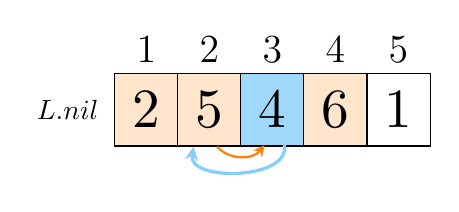
\begin{tikzpicture}
			\node at (-1,0) {$L.nil$};
			\node(2) at (0,0)[text=black,fill=orange!20,label=\Large1,draw,scale=2]{2};
			\node(5) at (0.8,0)[text=black,fill=orange!20,label=\Large2,draw,scale=2]{5};
			\node(4) at (1.6,0)[text=black,fill=skyblue!80,label=\Large 3,draw,scale=2]{4};
			\node(6) at (2.4,0)[text=black,fill=orange!20,label=\Large 4,draw,scale=2]{6};
			\node(1) at (3.2,0)[text=black,label=\Large 5,draw,scale=2]{1};
			
			\draw[->,>=stealth,very thick,skyblue,bend left=100](1.75,-0.45) to (0.6,-0.47);
			\draw[->,>=stealth,thick,orange,bend angle=50,bend right](0.9,-0.47) to (1.5,-0.45); 
		\end{tikzpicture}
		
		\subsection{Practice 03:}
\begin{lstlisting}
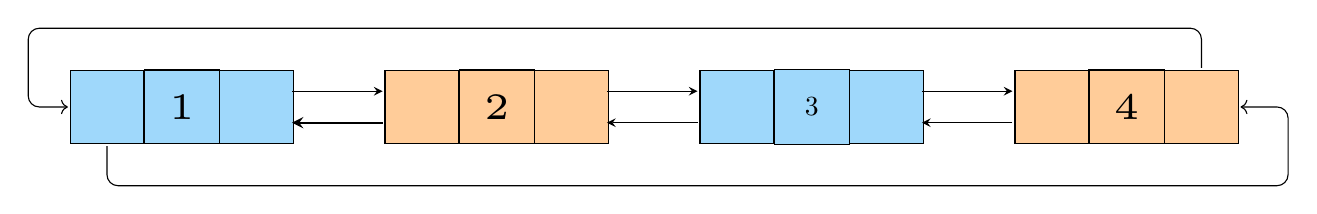
\begin{tikzpicture}
	\node(0) at (0,0)[text=black,fill=skyblue!80,draw,scale=4]{};
	\node at (0.95,0)[text=black,fill=skyblue!80,draw,scale=2.7]{\tiny1};
	\node(1) at (1.9,0)[text=black,fill=skyblue!80,draw,scale=4]{};
			
	\node(2) at (4,0)[text=black,fill=orange!40,draw,scale=4]{};
	\node at (4.95,0)[text=black,fill=orange!40,draw,scale=2.7]{\tiny2};
	\node(3) at (5.9,0)[text=black,fill=orange!40,draw,scale=4]{};
			
	\node(4) at (8,0)[text=black,fill=skyblue!80,draw,scale=4]{};
	\node at (8.95,0)[text=black,fill=skyblue!80,minimum width = 0.95cm, minimum height=0.95cm,draw,]{3};
	\node(5) at (9.9,0)[text=black,fill=skyblue!80,draw,scale=4]{};
			
	\node(6) at (12,0)[text=black,fill=orange!40,draw,scale=4]{};
	\node at (12.95,0)[text=black,fill=orange!40,draw,scale=2.7]{\tiny4};
	\node(7) at (13.9,0)[text=black,fill=orange!40,draw,scale=4]{};
			
			
	\draw[->,>=stealth,pos=1](2.35,0.2) to (3.5,0.2);
	\draw[->,>=stealth,thick] (3.5,-0.2)to(2.35,-0.2) ;
	\draw[->,>=stealth,pos=1](6.35,0.2) to (7.5,0.2);
	\draw[->,>=stealth,pos=1](7.5,-0.2) to (6.35,-0.2);
	\draw[->,>=stealth,pos=1](10.35,0.2) to (11.5,0.2);
	\draw[->,>=stealth,pos=1](11.5,-0.2) to (10.35,-0.2);
			
	\draw[->, rounded corners](0.south) to(0,-1)to(15,-1) to (15,0)to(7.east);
	\draw[->, rounded corners](7.north) to(13.9,1)to(-1,1) to (-1,0)to(0.west);
\end{tikzpicture}
\end{lstlisting}


		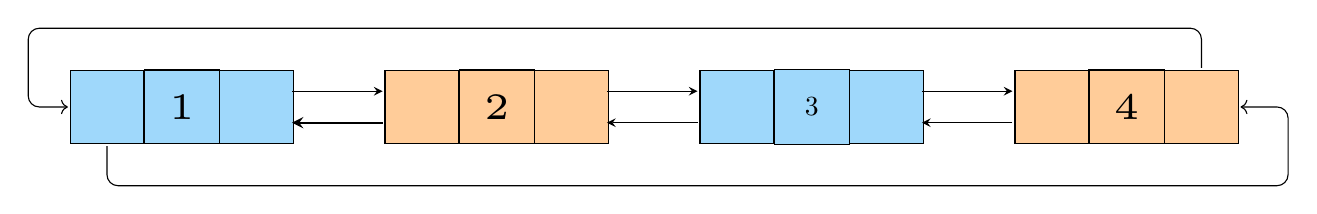
\begin{tikzpicture}
			\node(0) at (0,0)[text=black,fill=skyblue!80,draw,scale=4]{};
			\node at (0.95,0)[text=black,fill=skyblue!80,draw,scale=2.7]{\tiny1};
			\node(1) at (1.9,0)[text=black,fill=skyblue!80,draw,scale=4]{};
			
			\node(2) at (4,0)[text=black,fill=orange!40,draw,scale=4]{};
			\node at (4.95,0)[text=black,fill=orange!40,draw,scale=2.7]{\tiny2};
			\node(3) at (5.9,0)[text=black,fill=orange!40,draw,scale=4]{};
			
			\node(4) at (8,0)[text=black,fill=skyblue!80,draw,scale=4]{};
			\node at (8.95,0)[text=black,fill=skyblue!80,minimum width = 0.95cm, minimum height=0.95cm,draw,]{3};
			\node(5) at (9.9,0)[text=black,fill=skyblue!80,draw,scale=4]{};
			
			\node(6) at (12,0)[text=black,fill=orange!40,draw,scale=4]{};
			\node at (12.95,0)[text=black,fill=orange!40,draw,scale=2.7]{\tiny4};
			\node(7) at (13.9,0)[text=black,fill=orange!40,draw,scale=4]{};
			
			
			\draw[->,>=stealth,pos=1](2.35,0.2) to (3.5,0.2);
			\draw[->,>=stealth,thick] (3.5,-0.2)to(2.35,-0.2) ;
			\draw[->,>=stealth,pos=1](6.35,0.2) to (7.5,0.2);
			\draw[->,>=stealth,pos=1](7.5,-0.2) to (6.35,-0.2);
			\draw[->,>=stealth,pos=1](10.35,0.2) to (11.5,0.2);
			\draw[->,>=stealth,pos=1](11.5,-0.2) to (10.35,-0.2);
			
			\draw[->, rounded corners](0.south) to(0,-1)to(15,-1) to (15,0)to(7.east);
			\draw[->, rounded corners](7.north) to(13.9,1)to(-1,1) to (-1,0)to(0.west);
		\end{tikzpicture}
		
%--------------------------------- Practice 04-------------------------------------------
\pagebreak		
\subsection{Practice 04:}		
	\begin{figure}[h!]
	\centering
		\fbox{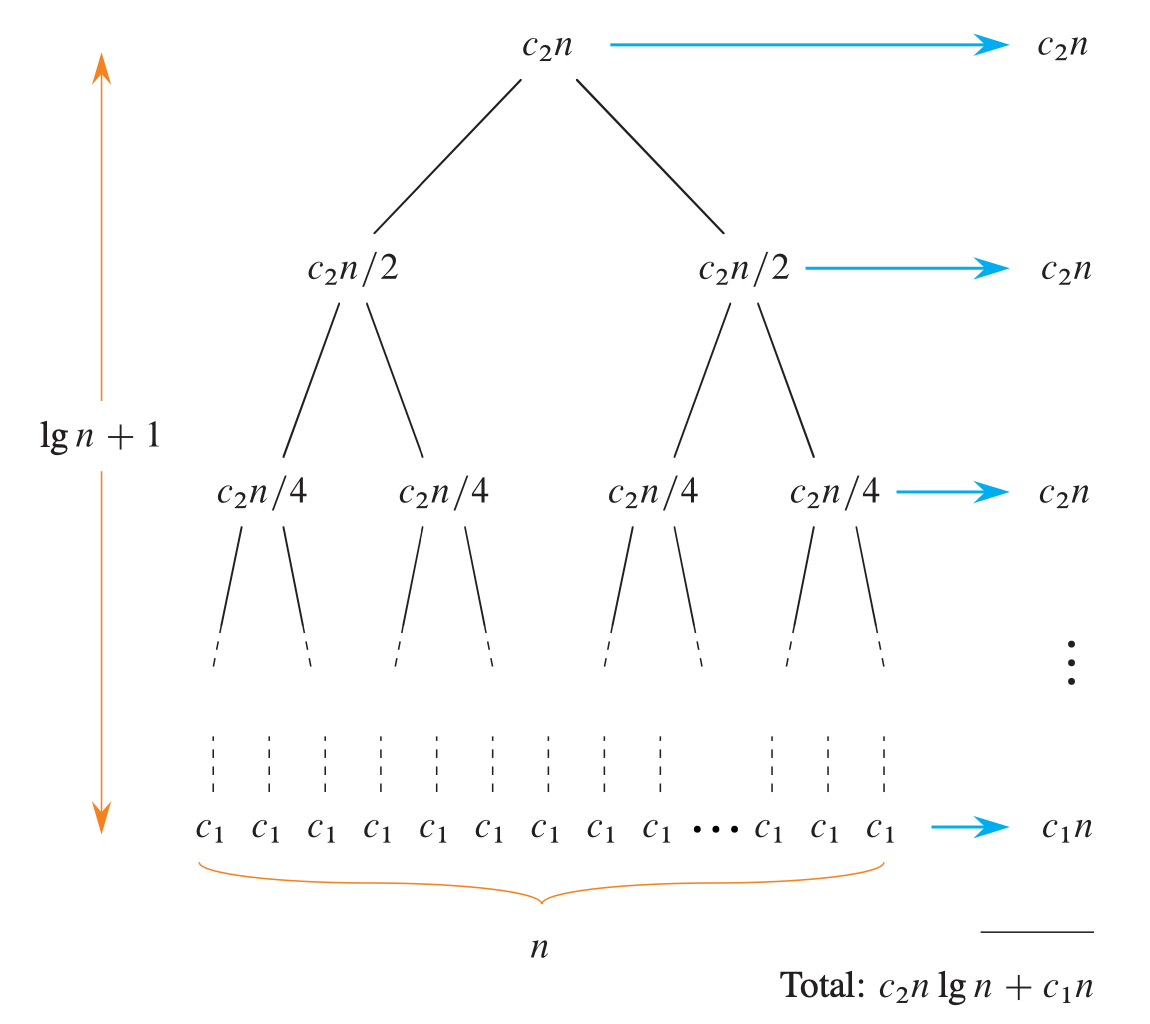
\includegraphics[width=0.7\textwidth]{./6.png}}
		\caption{Reference}
    		\label{fig:border}
	\end{figure}
                       %-----x------%	
	\begin{center} 	
	\begin{tikzpicture}[
		level 1/.style={level distance = 25mm, sibling distance = 40mm}, 
		level 2/.style={level distance = 25mm, sibling distance = 20mm},
		level 3/.style={sibling distance = 10mm}]
		\node {$c_2n$}
			child {node{$c_2n/2$}
				child{node{$c_2n/4$}
					 child{node(1){}}
					 child{node(2){}}
				}
				child{node{$c_2n/4$}
					child{node(3){}}
					child{node(4){}}				
				}
			}
			child {node{$c_2n/2$}
				child{node{$c_2n/4$}
					child{node(5){}}
					child{node(6){}}				
				}
				child{node{$c_2n/4$}
					child{node(7){}}
					child{node(8){}}				
				}
			};
			\foreach \i/\j in {1/2,3/4,5/6,7/8}{
				\draw[-,dashed] (\i) to ($(\i)+(-0.05,-0.5)$);
				\draw[-,dashed] (\j) to ($(\j)+(0.05,-0.5)$);
				\draw[dashed] ($(\i)+(-0.05,-1)$) to ($(\i)+(-0.045,-2)$)node [below]{$c_1$};
				\draw[dashed] ($(\j)+(0.05,-1)$) to ($(\j)+(0.05,-2)$)node [below]{$c_1$};
				\draw[dashed] ($((\i)+(-0.05,-1))!0.5!((\j)+(0.05,-1))$) to ($((\i)+(-0.045,-2))!0.5!((\j)+(0.05,-2))$);			
			}
			\draw[rounded corners=10pt, thick]
    				($(1)!0.5!(8) + (0,-3.5)$)
    				-- ++ (-0.5,0.5)
    				--
    				($(1)+(-0.2,-3)$)
    				--
    				($(1)+(-0.2,-2.5)$);			
			
			 \draw[rounded corners=10pt, thick]
    				($(1)!0.5!(8) + (0,-3.5)$)
    				-- ++ (0.5,0.5)
    				--
    				($(8)+(0.2,-3)$)
    				--
    				($(8)+(0.2,-2.5)$);
			\node at ($(1)!0.5!(8) + (0,-3.5)$) [below] {$n$};
	\end{tikzpicture}
	\end{center}
\end{document}